\section{Results}
%-------------------------------------------------------------------------------------------------------------
% Acceleration
The vertical acceleration of the sprung mass $\Ddot{z}_s$ remained below $1.5\frac{\text{m}}{\text{s}^2}$ during the entire simulation except for two spikes at the very roughest parts (see Table.\:\ref{tab:tests}), see Fig.\:\ref{fig:vertical_acceleration}.
\begin{figure}
    \centering
    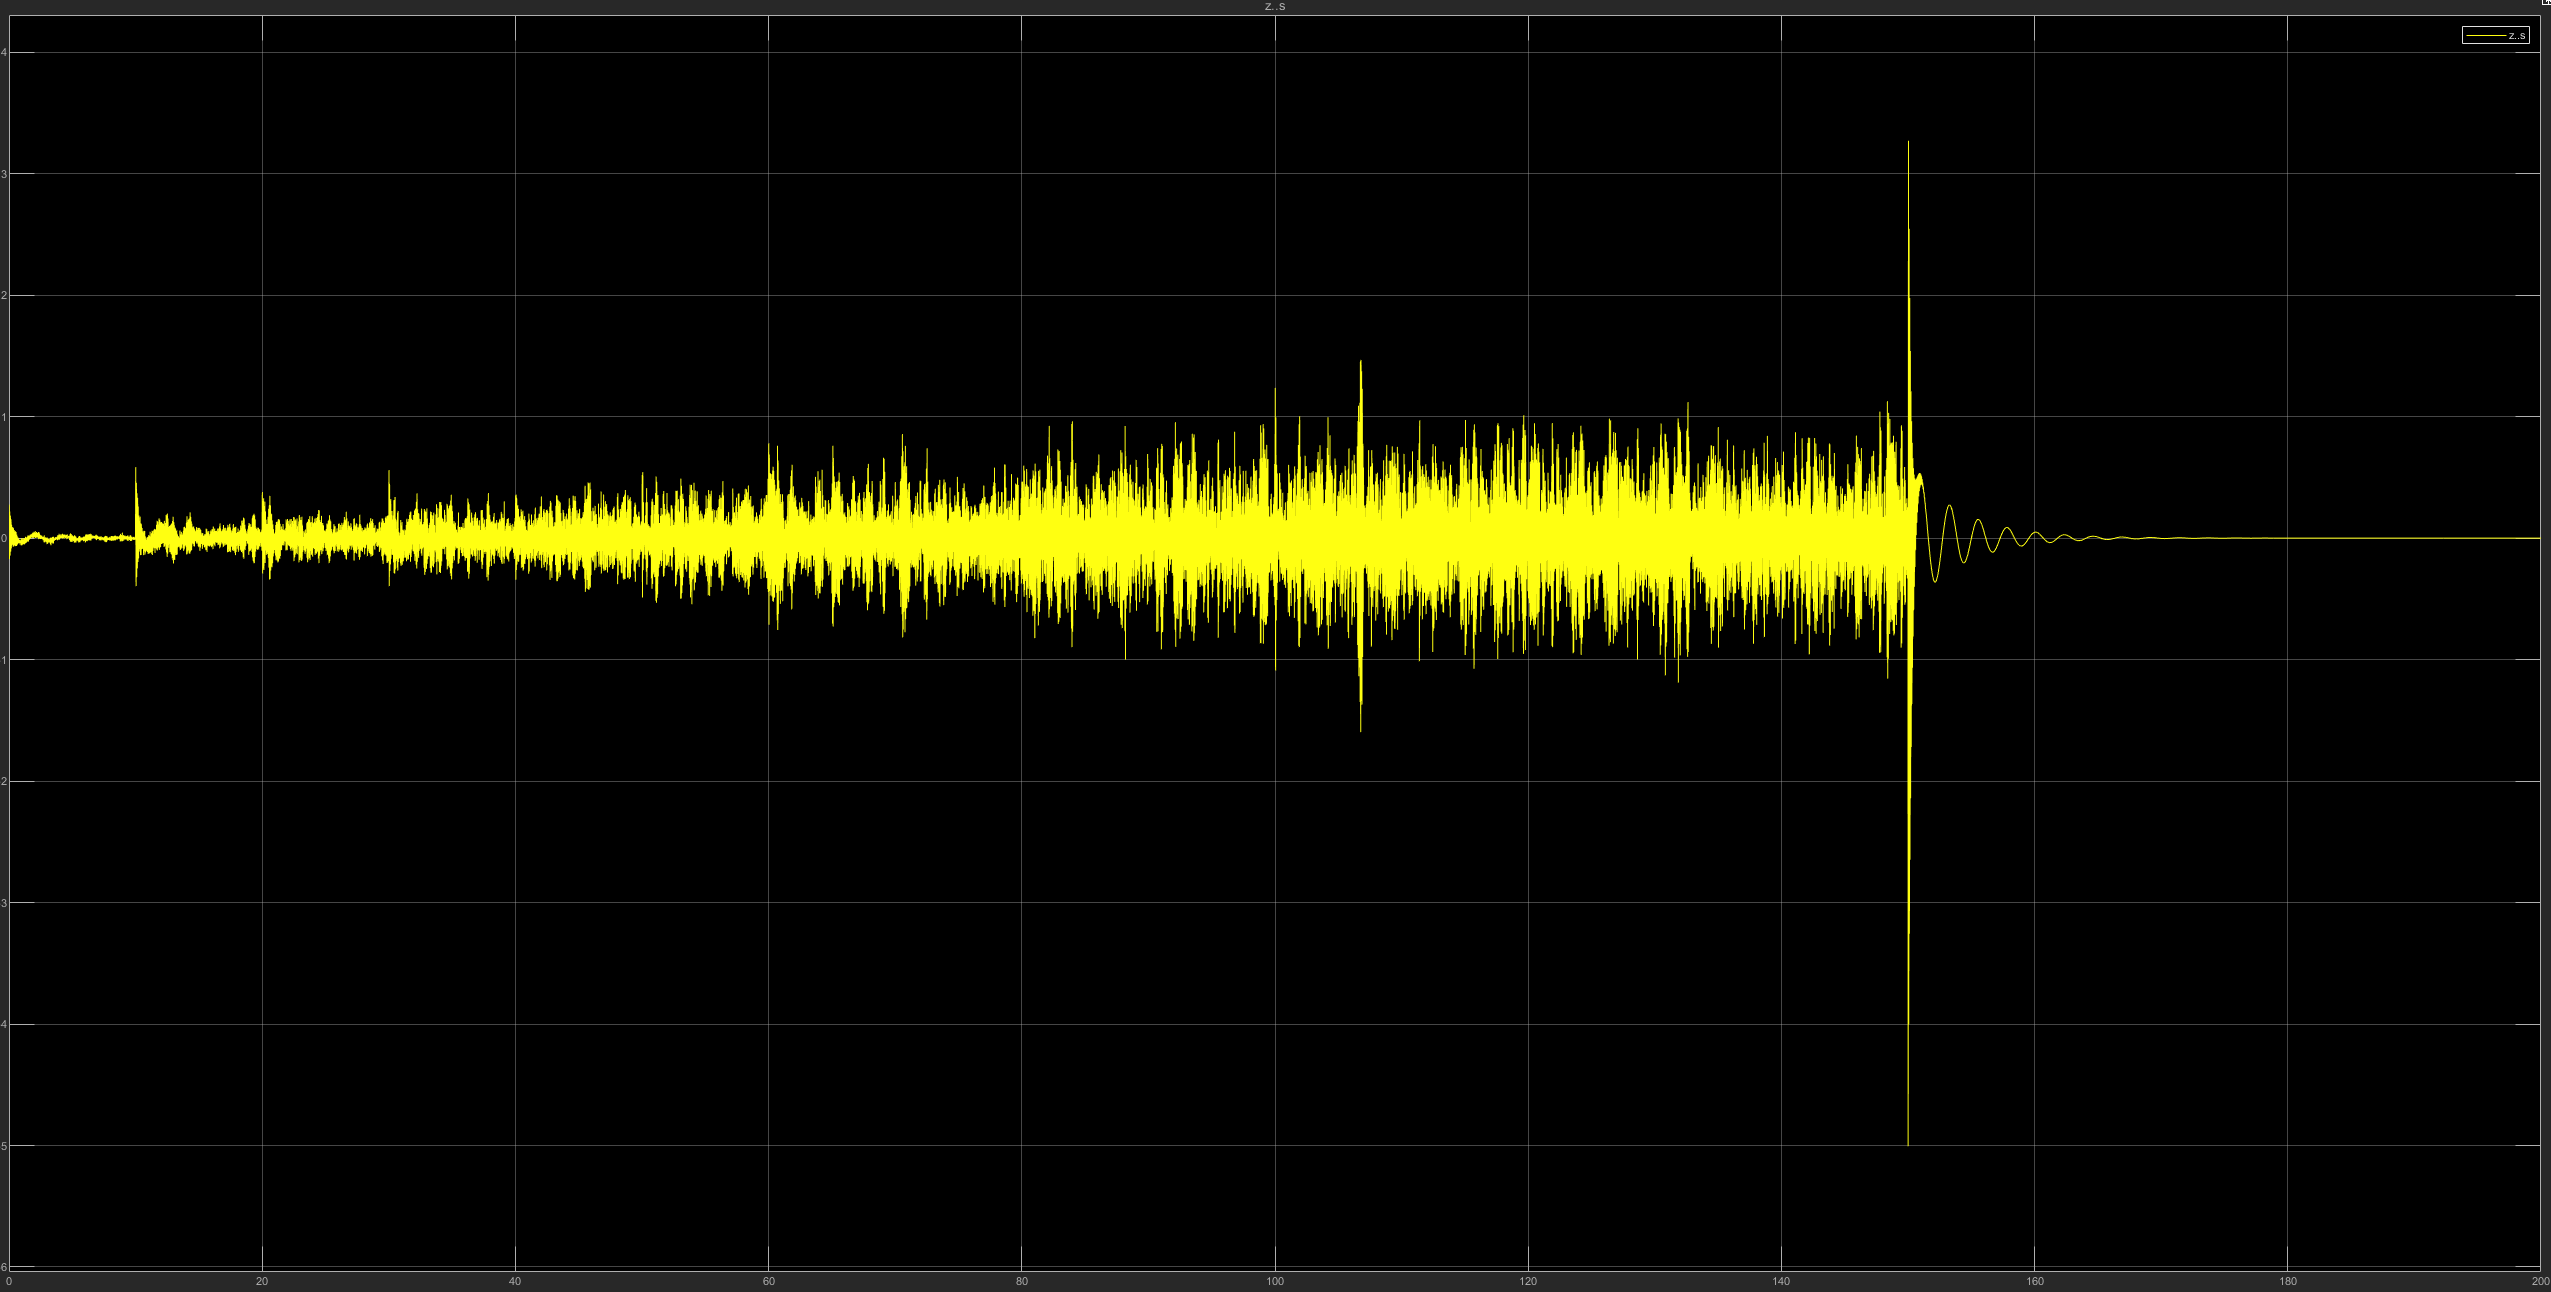
\includegraphics[width=\columnwidth]{images/vertical_acceleration.png}
    \caption{Simulation results of the vertical acceleration of the sprung mass.}
    \label{fig:vertical_acceleration}
\end{figure}

% Energy
The energy results obtained, when the simulated model was subjected to the noise input described in \eqref{eq:noise} and Table.\:\ref{tab:tests}, can be seen in Table.\:\ref{tab:results_energy}, Fig.\:\ref{fig:energy_results_graph} and Fig.\:\ref{fig:self_supplying}.
\begin{table}[ht]
	\centering
	\begin{tabular}{|l|l|l|l|l|l|}
			\hline
			Metric                                            & Proposed RASS        \\
			\hline
			Energy consumed (J)                               & $-6760$               \\
			Energy regenerated (J)                            & $5650$               \\
			Total energy consumed/regenerated (J)             & $-1110$               \\
            Self supplying efficiency (\%)                    & $88$             \\
			\hline
		\end{tabular}
	\caption{All energy values obtained from the simulation.}
	\label{tab:results_energy}
\end{table}

\begin{figure}
    \centering
    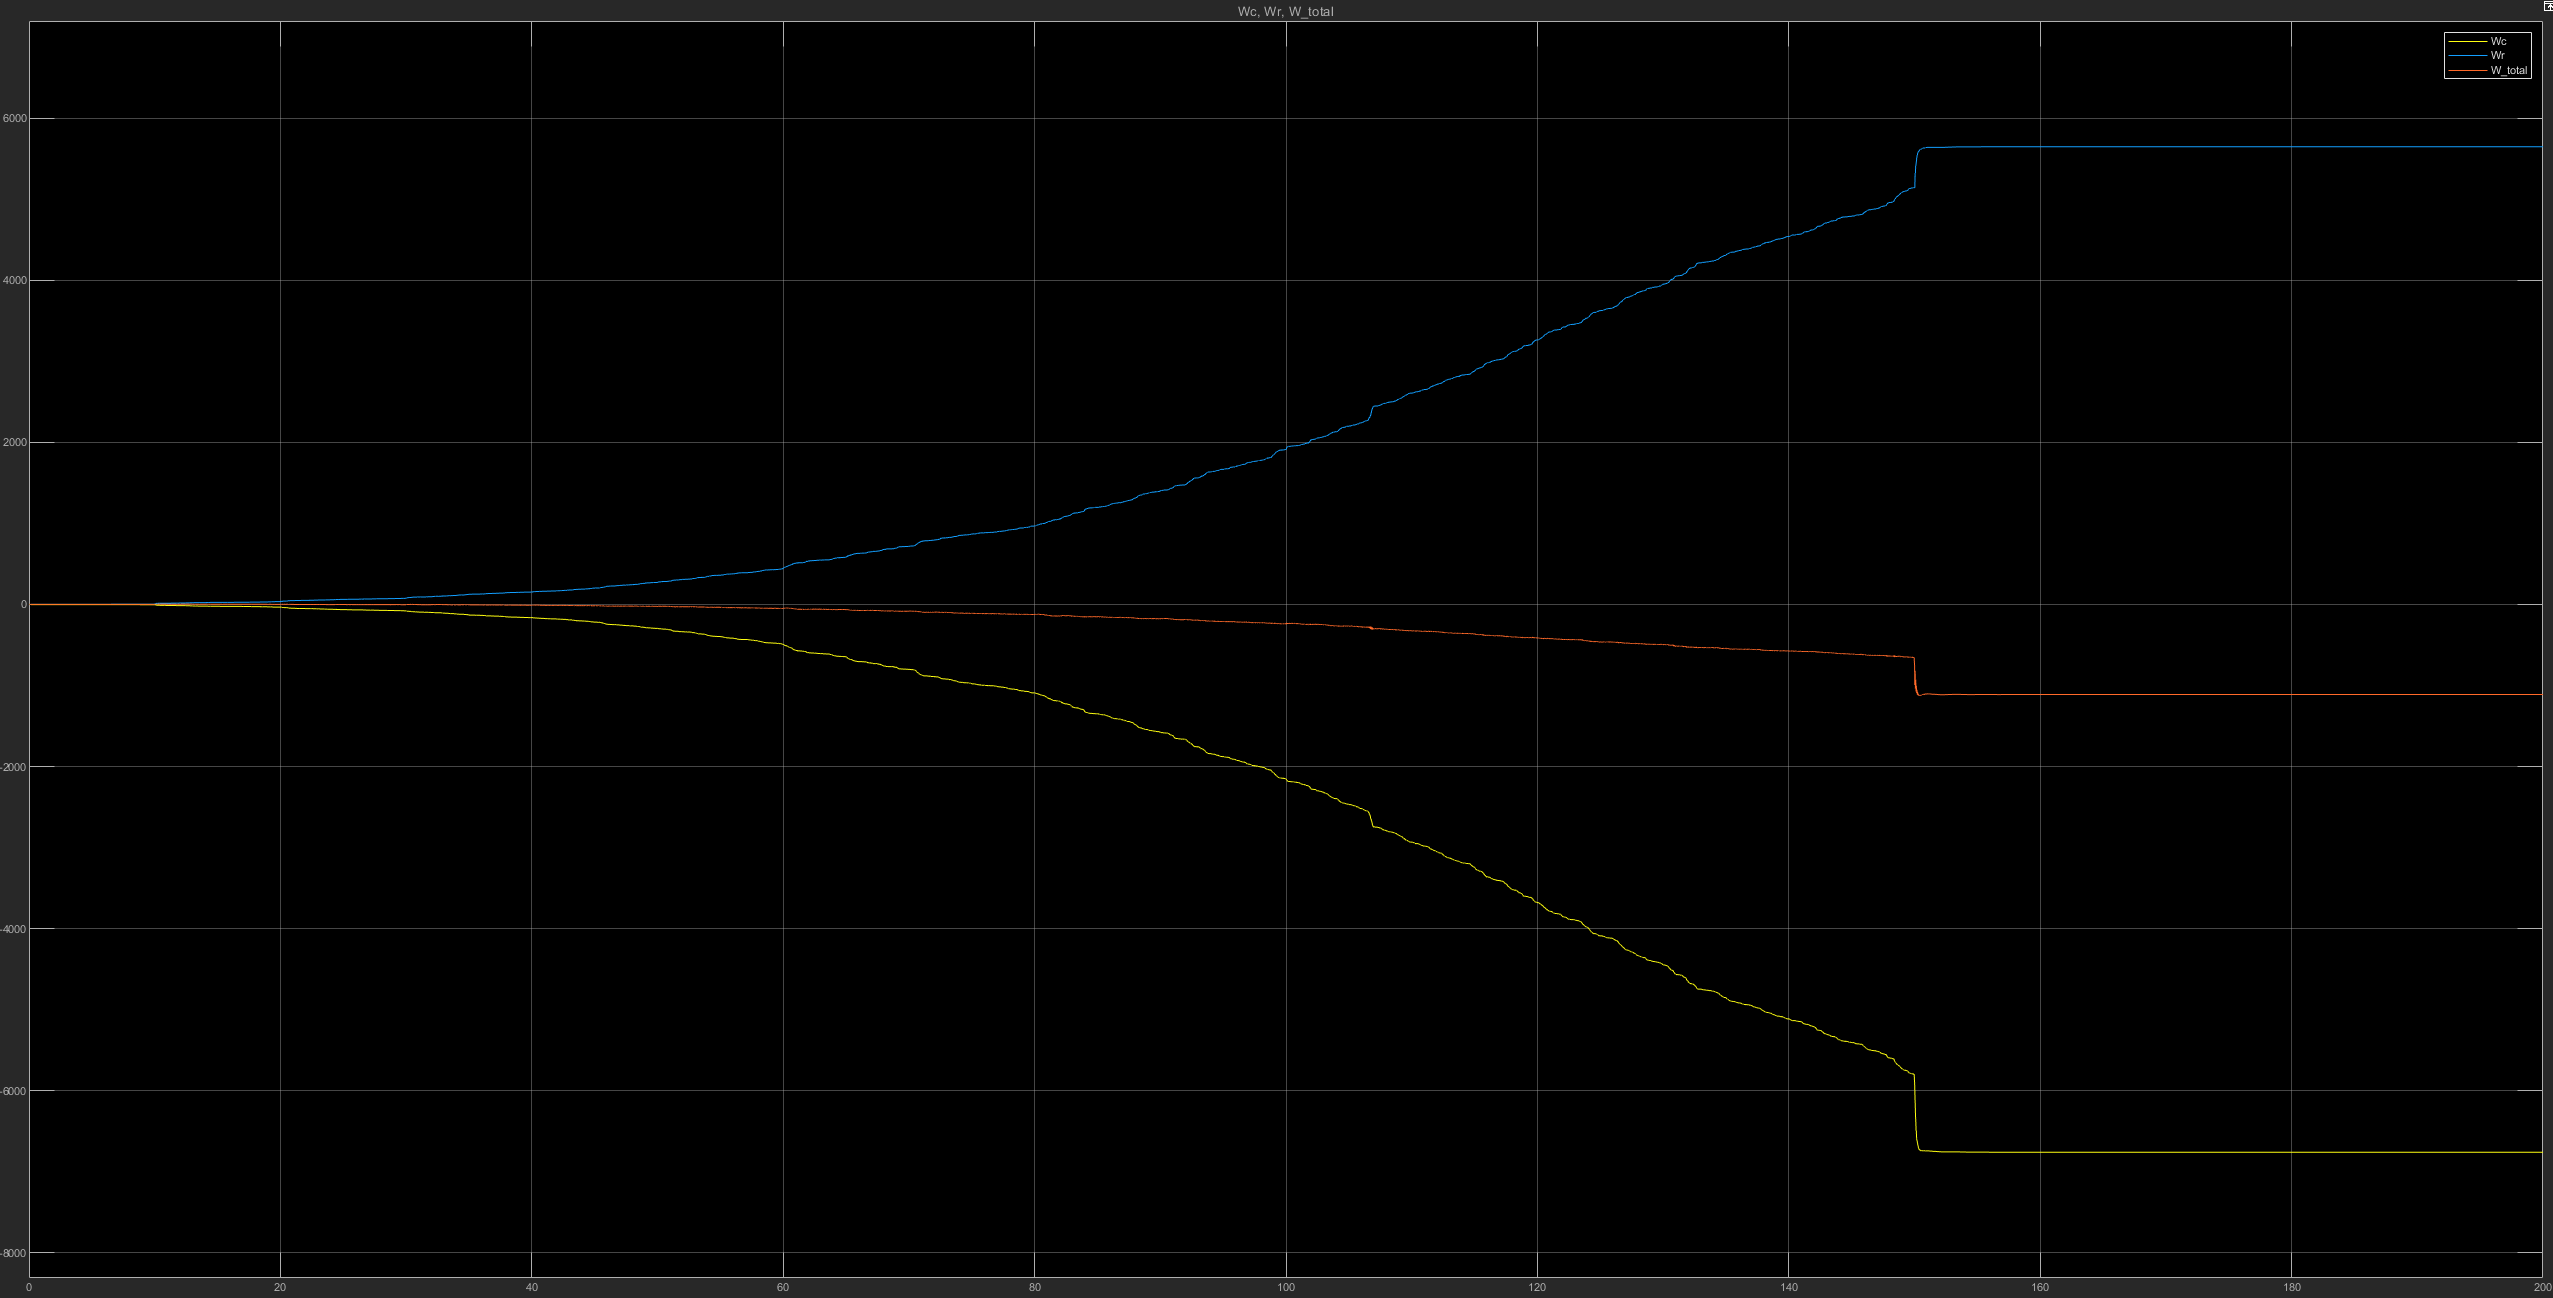
\includegraphics[width=\columnwidth]{images/energy_results.png}
    \caption{Simulation results of the energy consumed, regenerated and total energy. Yellow line is energy consumed, blue line is energy regenerated and red line is total energy.}
    \label{fig:energy_results_graph}
\end{figure}

\begin{figure}
    \centering
    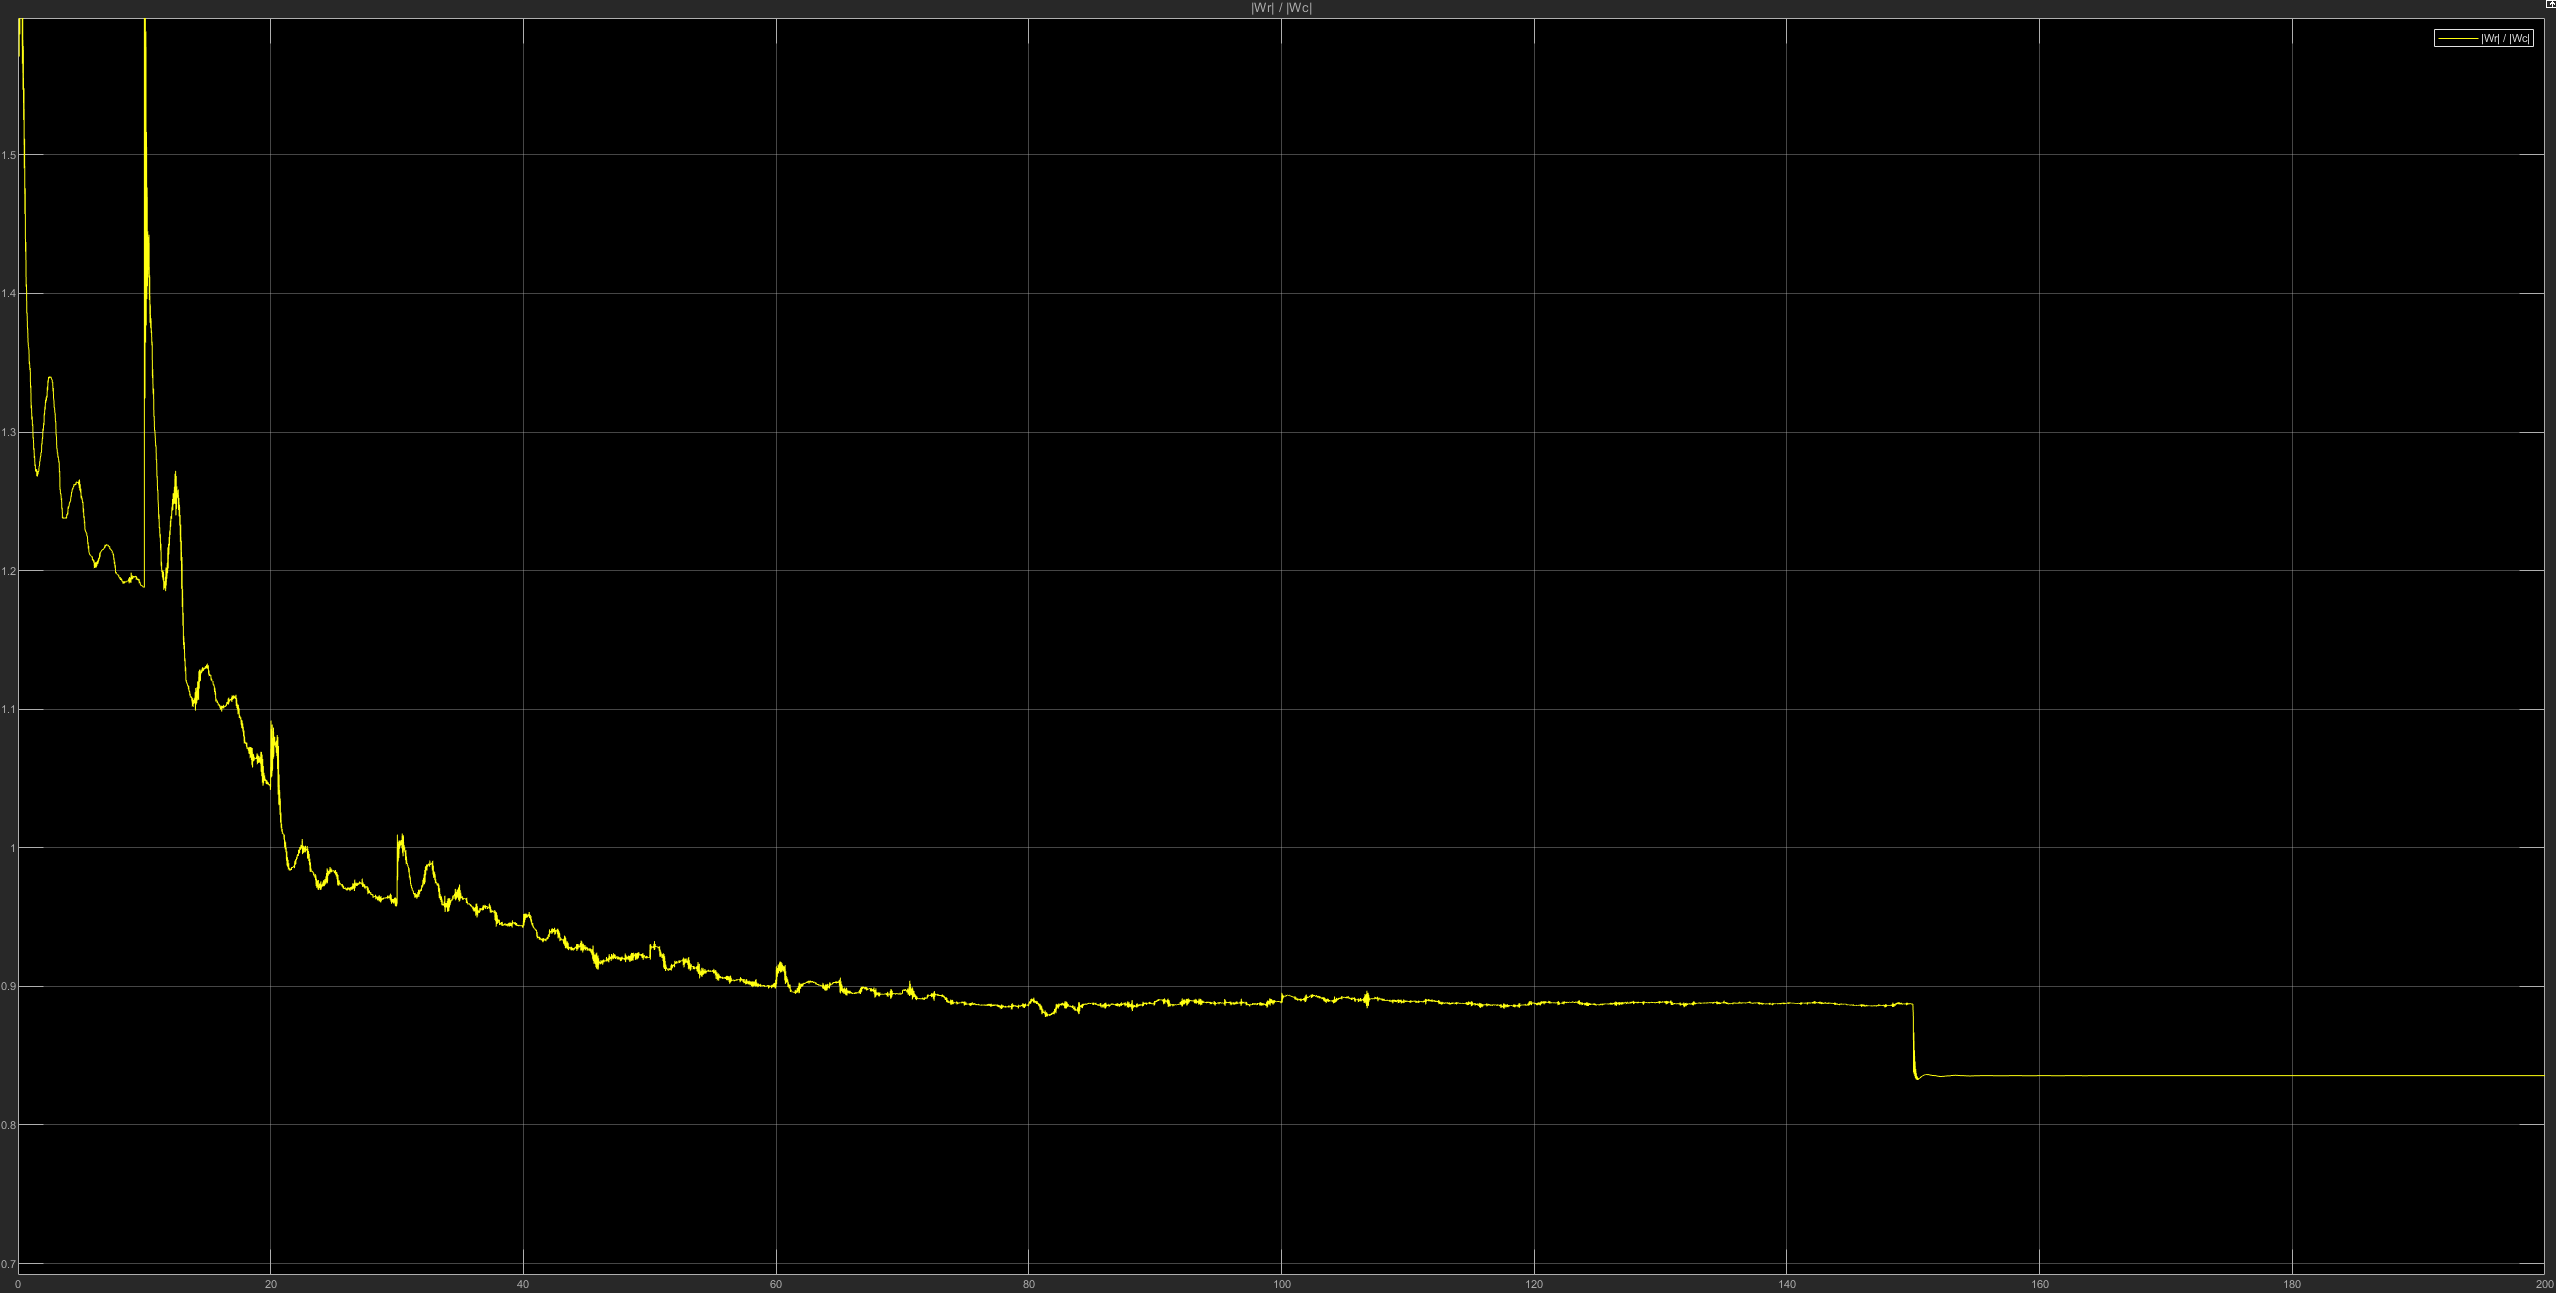
\includegraphics[width=\columnwidth]{images/self_supplying.png}
    \caption{Simulation results of the self supplying efficiency.}
    \label{fig:self_supplying}
\end{figure}

A number of requirements could not be evaluated, including energy efficiency.
%-------------------------------------------------------------------------------------------------------------